\documentclass[border=10pt]{standalone}

\usepackage{tikz}
\usepackage{tikzsymbols}
\usetikzlibrary{calc,patterns,shapes.geometric}

\def\centerarc[#1](#2)(#3:#4:#5){\draw[#1] ($(#2)+({#5*cos(#3)},{#5*sin(#3)})$) arc (#3:#4:#5);}

\begin{document}
	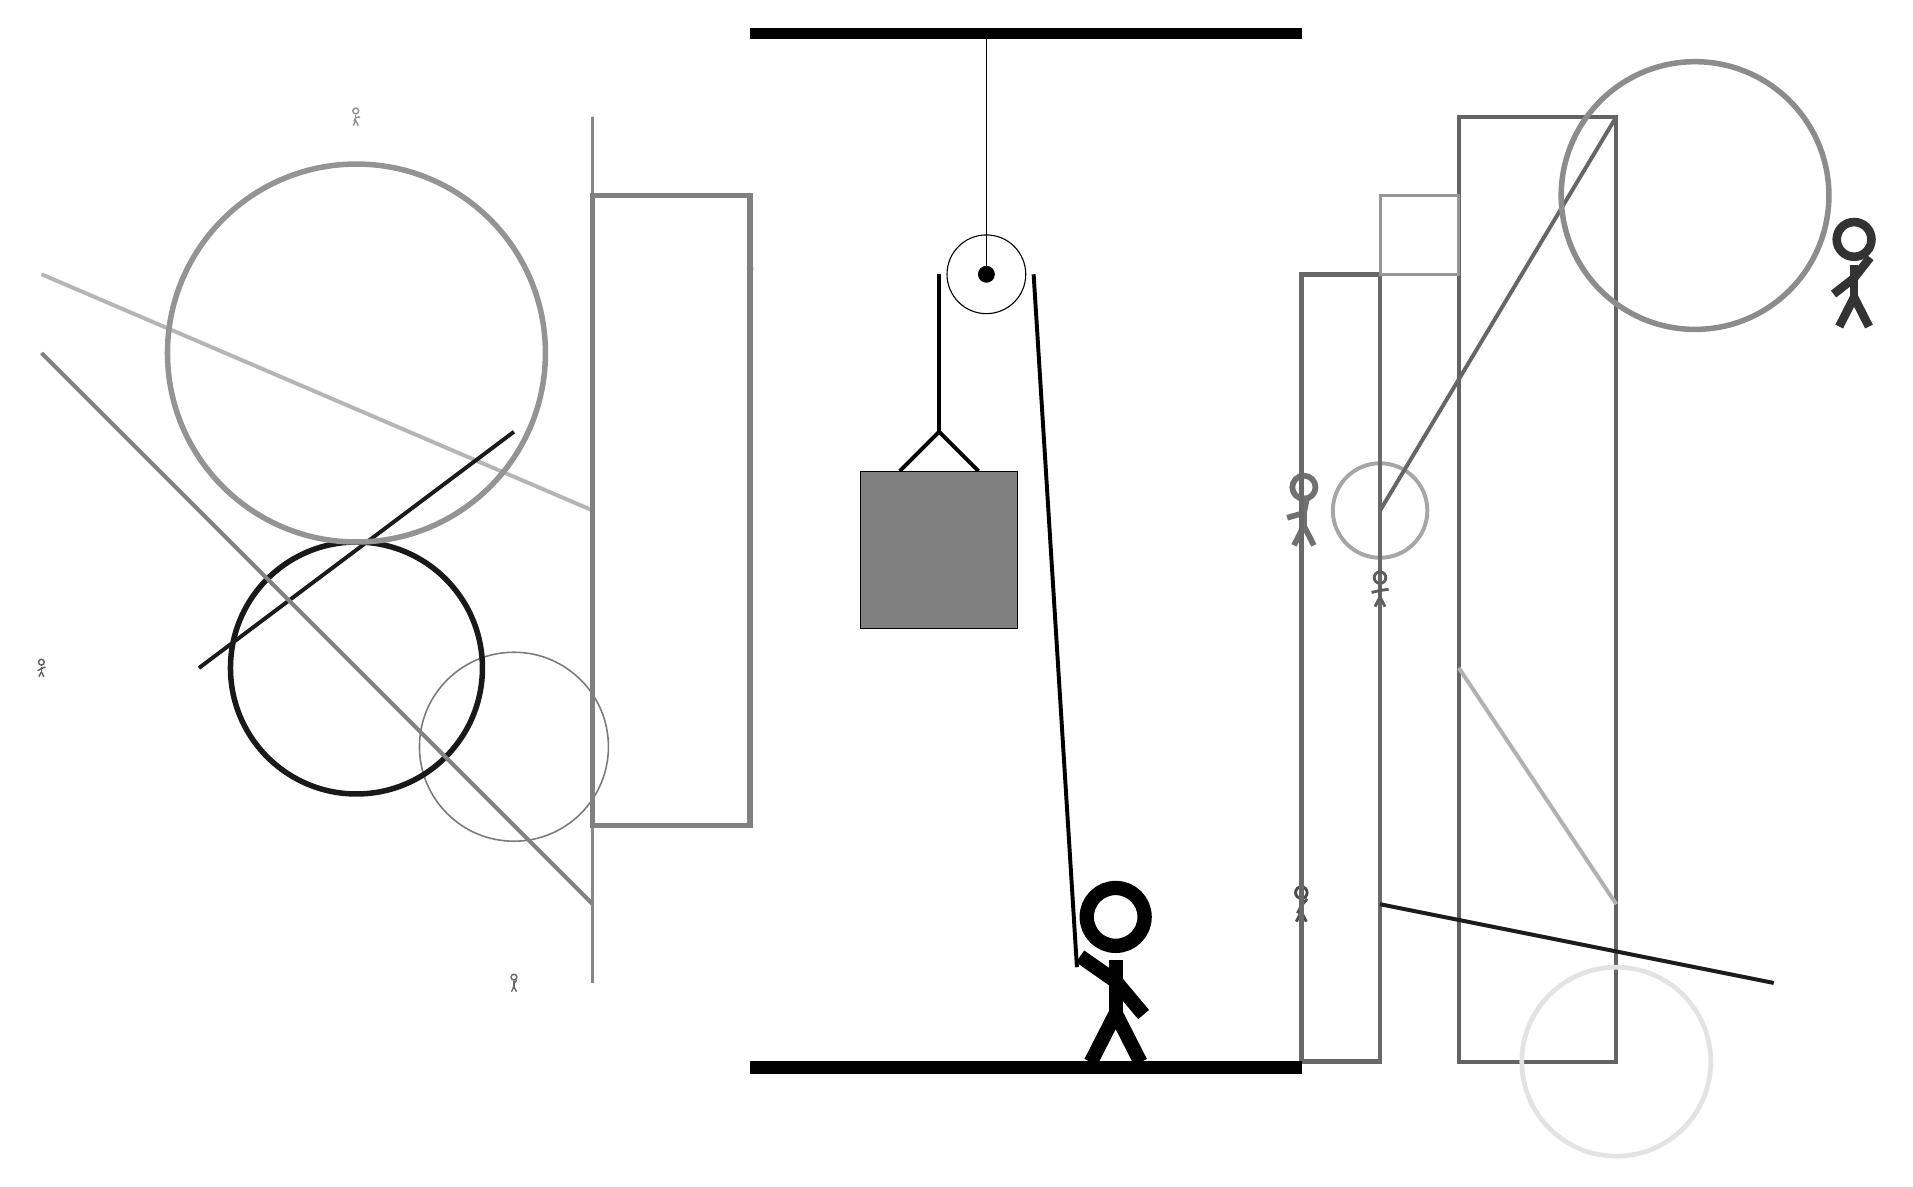
\begin{tikzpicture}
		%%%%% START %%%%%
		
		\draw[fill=black] (-2, 10) rectangle (5, 10.125);
		
		\draw (1, 7) circle (0.5);
		\draw[fill=black] (1, 7) circle (0.1);
		\draw (1, 10) -- (1, 7);
		
		\draw[line width=0.5mm] (-0.1, 4.5) -- (0.4, 5.0) -- (0.9, 4.5);
		\draw[fill=black!50] (-0.6, 4.5) rectangle (1.4, 2.5);
		
		\draw[line width=0.5mm] (0.4, 7) -- (0.4, 5.0);
		\centerarc[line width=0.5mm](1, 7)(0:180:0.6);
		\draw[line width=0.5mm](1.6, 7) -- (2.15, -1.8);
		
		\node at (2.6, -1.9) {\Strichmaxerl[10][-35][-50]};
		
		\draw[line width=0.5mm, color=black!61] (7, 9) rectangle (9, -3);
		
		\draw [line width=0.5mm, color=black!35](6, 4) circle (0.6);
		\node[line width=0.4mm, color=black!62] at (-11, 2) {\Strichmaxerl[1][29][23]};
		\node[line width=0.3mm, color=black!80] at (12, 7) {\Strichmaxerl[6][38][52]};
		\draw [line width=0.2mm, color=black!52](-5, 1) circle (1.2);
		\draw[line width=0.5mm, color=black!29](-4, 4) -- (-11, 7);
		\node[line width=0.5mm, color=black!59] at (-5, -2) {\Strichmaxerl[1][83][49]};
		\draw[line width=0.5mm, color=black!60](9, 9) -- (6, 4);
		\draw [line width=0.6mm, color=black!11](9, -3) circle (1.2);
		\draw[line width=0.3mm, color=black!39] (-4, 9) rectangle (-4, 0);
		
		\node[line width=0.2mm, color=black!44] at (-7, 9) {\Strichmaxerl[1][63][5]};
		\draw [line width=0.7mm, color=black!45](10, 8) circle (1.7);
		\node[line width=0.2mm, color=black!71] at (5, -1) {\Strichmaxerl[2][64][48]};
		
		\draw [line width=0.7mm, color=black!90](-7, 2) circle (1.6);
		\draw[line width=0.4mm, color=black!47] (-4, 9) rectangle (-4, -2);
		\node[line width=0.2mm, color=black!56] at (5, 4) {\Strichmaxerl[4][16][78]};
		\draw[line width=0.6mm, color=black!59] (6, -3) rectangle (5, 7);
		\draw[line width=0.5mm, color=black!89](-5, 5) -- (-9, 2);
		\draw [line width=0.7mm, color=black!42](-7, 6) circle (2.4);
		\draw[line width=0.5mm, color=black!49](-4, -1) -- (-11, 6);
		\draw[line width=0.5mm, color=black!31](7, 2) -- (9, -1);
		\node[line width=0.6mm, color=black!63] at (6, 3) {\Strichmaxerl[2][13][8]};
		
		\draw[line width=0.5mm, color=black!89](6, -1) -- (11, -2);
		\node[line width=0.3mm, color=black!20] at (-2, 7) {\Strichmaxerl[1][50][76]};
		\draw[line width=0.4mm, color=black!41] (6, 8) rectangle (7, 7);
		
		\draw[line width=0.7mm, color=black!50] (-2, 0) rectangle (-4, 8);
		
		\draw[fill=black] (-2, -3) rectangle (5, -3.15);
		
		%%%%% END %%%%%
	\end{tikzpicture}
\end{document}